\documentclass{beamer}

\usepackage{ucs}  %UTF-8
\usepackage[utf8]{inputenc} %UTF-8

\usepackage[ngerman]{babel}%deutsch

\usepackage{amsmath,amssymb,amstext}%mathe

\usepackage{graphicx}%grafik einbinden

\usepackage[amssymb]{SIunits}%si-interpreter

\usepackage{marvosym}%nützliche symbole, z.B.\EUR

\usepackage{pdfpages}% pdf seiten einbinden

\usepackage{float} %Grafikpositionierung erzwingen

\usepackage{alphabeta}  %griechisch im Text-Modus

\usepackage{url}%URL mit zeilenumbruch und andere schrift

\usepackage{makecell}

%\setlength\abovecaptionskip{-3pt}

\usepackage{enumerate}

\usepackage[font=tiny]{caption}

\usetheme{default}%uni-theme

\title{Mechanismen annormaler Diffusion}
\author[J. Mihatsch]{Jakob Mihatsch}
\institute{Universität Greifswald}%fußzeile
\date{15.01.2021}
\setbeamertemplate{footline}{\hfill \insertframenumber/\inserttotalframenumber}

\addtobeamertemplate{frametitle}{\vspace*{0cm}}{\vspace*{-0.6cm}}

\begin{document}
	\begin{frame}
		\titlepage
	\end{frame}
\begin{frame}
	\frametitle{Inhalt}
	\tableofcontents
\end{frame}
\section{Diffusion}
{ % these braces make the change local to the single frame
\setbeamertemplate{footline}{Gardiner 1985, Demtröder 2006 \hfill \insertframenumber/\inserttotalframenumber}
	\begin{frame}
		\frametitle{Grundlagen der Diffusion}
		\begin{itemize}
			\item Robert Brown 1827: Bewegung von Pflanzensamen in wässriger Lösung
			\item Phänomenologischer Ansatz: Ficksche Gesetze \\
			$\mathbf{J} = -D \nabla c $ (1. Ficksches Gesetz) \\
			$\frac{\partial c}{\partial t} = -\nabla \mathbf{J} $ (Kontinuitätsgleichung) \\
			$\rightarrow$ $\boxed{\frac{\partial c}{\partial t} = D \Delta c}$ (Diffusionsgleichung/2. Ficksches Gesetz)
			
			\item Später durch Einstein von mikroskopischen Prinzipien hergeleitet
			\item mittlere quadratische Abweichung\\
			$c(x, t) = \frac{1}{\sqrt{4\pi D t}}\exp(-\frac{x^2}{4Dt})$ \\(in 1D, für $\delta$-förmige Anfangsbed.)\\
			$\boxed{\left<x^2\right> = 2Dt}$
		\end{itemize}
	\end{frame}
}
	\begin{frame}
		\frametitle{Random Walk}
		\begin{equation*}x_t = x_0 + \sum_{j=1}^n \sigma_j\end{equation*}
		$\sigma_j$ unabhängige Zufallsvariablen
		\begin{equation*}\left<x^2\right> = \left< \left(x_0 + \sum_{j=1}^t \sigma_j\right)^2 \right> = \end{equation*}
		mit $x_0=0$ und $\sigma_i = \pm \sqrt{2D}$ mit gleicher Wahrscheinlichkeit:
		\begin{eqnarray*} = &\sum_{j=1}^t \left<\sigma_j^2\right> &+ \sum_{j=1}^t \sum_{i\neq j} \left<\sigma_j \sigma_i\right> \\
		= &2Dt &+ 0 \end{eqnarray*}
		\begin{figure}
			\raggedleft
			\vspace*{-1cm}
			\includegraphics[width=.3\textwidth]{Literatur/480px-BrownianMotion.svg.png}
			\caption{Random Walk mit 1000 Schritten (User:PAR, Public domain, via Wikimedia Commons)}
		\end{figure}
	\end{frame}
{ % these braces make the change local to the single frame
\setbeamertemplate{footline}{Klafter \& Sokolov 2005  \hfill \insertframenumber/\inserttotalframenumber}
\section{Annomale Diffusion: Definition}
	\begin{frame}
		\frametitle{Annomale Diffusion}
		Verallgemeinerung: 
		\begin{equation*}
			\left< x^2 \right> \propto t^\alpha
		\end{equation*}
		man unterscheidet die Fälle
		\begin{equation*}
			\begin{cases}
				\alpha < 1 & \text{Subdiffusion} \\
				\alpha = 1 & \text{normale Diffusion} \\
				\alpha > 1 & \text{Superdiffusion} \\
				\alpha = 2 & \text{ballistisches Verhalten}
			\end{cases}
		\end{equation*}
	\end{frame}
}
	\section{Annormale Diffusion: Beispiele}
	\subsection{Subdiffusion in der Zellmembran}
	\begin{frame}
		\frametitle{Subdiffusion in der Zellmembran}
		\vspace*{0.5cm}
			\begin{figure}
				\centering
				\includegraphics[width=.8\textwidth]{Literatur/gr5_lrg.png}
				\caption{Hop Diffusion Trajektorien auf verschiedenen Zeitskalen (Ritchie et al., 2005)}
			\end{figure}
			\vspace*{-0.5cm}
			\begin{columns}
				\begin{column}{.5\textwidth}
					\begin{figure}
						\centering
						\includegraphics[width=.85\textwidth]{Literatur/MSD_hop.png}
						\caption{Mittlere quadratische Abweichung (MSD) für einzelne Hop Diffusion Trajektorie (Ritchie et al., 2005)}
					\end{figure}
				\end{column}
				\begin{column}{.5\textwidth}
					\begin{figure}
						\centering
						\includegraphics[width=\textwidth]{Literatur/Bildschirmfoto 2021-01-14 um 09.48.05.png}
						\caption{Fächerstruktur der Plasmamembran (Sako und Kusumi, 1996)}
					\end{figure}
				\end{column}
			\end{columns}
	\end{frame}
	\subsection{Tiere auf Nahrungssuche: Levy-Flight foraging hypothesis}
	\begin{frame}
		\frametitle{Levy-Flight foraging hypothesis}
		\begin{columns}[c]
			\begin{column}{.5\textwidth}
				\begin{figure}
					\centering
					\includegraphics[width=\textwidth]{saw/levvsexp.pdf}
					\caption{Vergleich von Normalverteilung und Levy-Verteilung (eigene Darstellung)}
				\end{figure}
				\begin{figure}
					\centering
					\includegraphics[width=.5\textwidth]{Literatur/500px-LevyFlight.svg.png}
					\caption{Levy-Flug mit 1000 Schritten (User:PAR, Public domain, via Wikimedia Commons)}
				\end{figure}
			\end{column}
			\begin{column}{.5\textwidth}
			\begin{figure}
				\centering
				\includegraphics[width=\textwidth]{Literatur/monkeysteps.png}
				\caption{Verteilung der Schrittweiten von Klammeraffen in einem 5min Intervall (Ramos-Fernandez et al., 2003)}
			\end{figure}
		\end{column}
		\end{columns}
	\end{frame}
	\begin{frame}
		\frametitle{Levy-Flight foraging hypothesis}
		\begin{columns}
			\begin{column}{0.6\textwidth}
				\begin{figure}
					\centering
					\includegraphics[width=\textwidth]{Tiere/vulture species_log.pdf}
					\caption{Mittlere quadratische Abweichung gemittelt über die Trajektorie von 162 Tagen eines Weißrückengeiers (eigene Berechnung, Daten von O. Spiegel et al., 2013)}
				\end{figure}
			\end{column}
			\begin{column}{0.4\textwidth}
				\begin{figure}
					\includegraphics[width=1.2\textwidth]{Tiere/vulture species_trajectory.pdf}
					\caption{Trajektorie (eigene Berechnung, Daten von O. Spiegel et al., 2013)}
				\end{figure}
				\begin{figure}
					\includegraphics[width=0.7\textwidth]{Tiere/White-backed_Vulture_Metrozoo_1.jpg}
					\caption{Weißrückengeier, Gyps africanus (Alexf, CC BY-SA 3.0, via Wikimedia Commons)}
				\end{figure}
			\end{column}
		\end{columns}
	\end{frame}
\subsection{Random Walk mit unendlichem Gedächtnis}
{ % these braces make the change local to the single frame
\setbeamertemplate{footline}{Schütz \& Trimper 2004 \hfill \insertframenumber/\inserttotalframenumber}
\begin{frame}
	\frametitle{Random-Walk mit Gedächtnis}
	Den Schritt $\sigma_{t+1}$ erhält man so:
	\begin{itemize}
		\item Wähle zufällig $t' \leq t$ mit Wahrscheinlichkeit $1/t$
		\item $\sigma_{t+1} = \begin{cases}
			\sigma_{t'} & \text{mit Wsk. } p \\
			-\sigma_{t'} & \text{mit Wsk. } 1-p
		\end{cases}$
		\item $\sigma_{1} = \begin{cases}
			1 & \text{mit Wsk. } q \\
			-1 & \text{mit Wsk. } 1-q
		\end{cases}$
	\end{itemize}
\end{frame}
\begin{frame}
	\frametitle{Random-Walk mit Gedächtnis}
	\begin{columns}[c]
		\begin{column}[]{.5\textwidth}
			\begin{figure}
				\centering
				\resizebox*{!}{\textwidth}{\includegraphics[width=\textwidth]{RW_mit_Gedächtnis/elefant_mean.png}}
				\caption{Mittlere Abweichung von zehntausend Läufern bei q = 0.8 und p = 0.3, 0.7 (eigene Berechnung)}
			\end{figure}
		\end{column}
		\begin{column}[]{.5\textwidth}
			\begin{figure}
				\centering
				\only<1>{\resizebox*{!}{.6\textwidth}{\includegraphics[width=\textwidth]{RW_mit_Gedächtnis/elefant-2.pdf}}}
				\only<2>{\resizebox*{!}{.6\textwidth}{\includegraphics[width=\textwidth]{RW_mit_Gedächtnis/elefant-1.pdf}}}
				\caption{Mittlere quadratische Abweichung von zehntausend Läufern bei q = 0.8 und p = 0.3, 0.7 (eigene Berechnung)}
			\end{figure}
		\end{column}
	\end{columns}
\end{frame}
\begin{frame}
	\frametitle{Random-Walk mit Gedächtnis}
	\begin{columns}[t]
		\begin{column}[]{.5\textwidth}
			\tiny
			\begin{equation*}
				\left\langle x_{t}^{2}\right\rangle=\frac{t}{2 \alpha-1}\left[\frac{\Gamma(t+2 \alpha)}{\Gamma(t+1) \Gamma(2 \alpha)}-1\right]
			\end{equation*}
			mit $\alpha = 2p-1$

			Asymptotisch:
			\begin{equation*}
				\begin{array}{c}
					\left\langle x_{t}^{2}\right\rangle\propto t, \quad p<3 / 4 \\ \quad\left\langle x_{t}^{2}\right\rangle\propto t \ln t, \quad p=3 / 4 \\
					\left\langle x_{t}^{2}\right\rangle\propto t^{4 p-2} , \quad p>3 / 4
					\end{array}
			\end{equation*}
			Die Wahrscheinlichkeitsdichte ist eine Gaußverteilung mit zeitabhängigem Diffusionskoeffizient
			\begin{equation*}
				P(x, t)=\frac{1}{\sqrt{4 \pi t D(t)}} \exp \left\{-\frac{[x-\bar{x}(t)]^{2}}{4 t D(t)}\right\}
			\end{equation*}
			wobei 
			\begin{equation*}
				D(t)=\frac{1}{4 \alpha-2}\left[\left(\frac{t}{t_{0}}\right)^{2 \alpha-1}-1\right]
			\end{equation*}
		\end{column}
		\begin{column}[]{.5\textwidth}
			\begin{figure}
				\centering
				\resizebox*{!}{.6\textwidth}{\includegraphics[width=\textwidth]{RW_mit_Gedächtnis/elefant.pdf}}
				\caption{Mittlere quadratische Abweichung von zehntausend Läufern bei q = 0.8 und p = 0.3, 0.7, 0.9 (eigene Berechnung)}
			\end{figure}
		\end{column}
	\end{columns}
\end{frame}
}
\section{Self-avoiding Walk}
\subsection{Problemstellung}
\begin{frame}
	\frametitle{Self-avoiding Random Walk (SAW)}
	\begin{columns}[t]
		\begin{column}{0.5\textwidth}
			\begin{figure}
				\centering
				\includegraphics[width=\textwidth]{saw/saw_ex.png}
				\caption{Self-avoiding Walk (eigene Darstellung)}
			\end{figure}
		\end{column}
		\begin{column}{0.5\textwidth}
			\begin{figure}
				\centering
				\includegraphics[width=\textwidth]{saw/saw_counterex.png}
				\caption{Normaler Random Walk (eigene Darstellung)}
			\end{figure}
		\end{column}
	\end{columns}
\end{frame}
\subsection{Flory-Exponent}
{ % these braces make the change local to the single frame
\setbeamertemplate{footline}{Madras \& Slade 2013,  Madras \& Sokal 1988\hfill \insertframenumber/\inserttotalframenumber}
\begin{frame}
	\frametitle{Flory-Exponent}
	\tiny
	Gehen aus vom normalen Random-Walk der Länge $N$
	\begin{equation*}
		\phi(\mathbf{R}, N)=\left(\frac{3}{2 \pi Nl^2}\right)^{3 / 2} \exp \left(-\frac{3 R^{2}}{2 Nl^2}\right)
	\end{equation*}
	Erhalte Entropie $S=-k_B \ln(W)$
	\begin{equation*}
		S(\mathbf{R})=S(0)-\frac{3}{2} k_{B} \frac{R^{2}}{N l^{2}}
	\end{equation*}
	Wechselwirkungsenergie zweier Monomere
	\begin{equation*}
		E_{\mid \mathrm{Mon}}=k_{B} T \nu
	\end{equation*}
	Multipliziere mit der mittleren Monomerzahl in Volumen $a^3$, wobei $a$ Ausdehnung eines Monomers ist, und der Anzahl der Monomere
	\begin{equation*}
		E \cong k_{B} T \nu \frac{N^{2} a^{3}}{R^{3}}
	\end{equation*}
	freie Energie $F=E-TS$
	\begin{equation*}
		F \cong k_{B} T\left[v \frac{N^{2} a^{3}}{R^{3}}+\frac{R^{2}}{N a^{2}}\right]
	\end{equation*}
	Minimieren der freien Energie liefert
	\begin{equation*}
		\frac{R}{N a^{2}} \cong \frac{N^{2} a^{3}}{R^{4}} \quad \text { oder } \quad \boxed{R \sim N^{3 / 5}}
	\end{equation*}
\end{frame}
\begin{frame}
	\frametitle{Flory-Exponent}
	\begin{columns}[t]
		\begin{column}{0.5\textwidth}
			\begin{equation*}
				\left<R(n)^2\right> \propto N^{2\nu}
			\end{equation*}
			\begin{equation*}
				\nu = \begin{cases}
					\frac{3}{4} & d=2 \\
					\frac{3}{5} & d=3 \\
					\frac{1}{2} & d \geq 4
				\end{cases}
			\end{equation*}
			Genaue Rechnungen liefern
			\begin{equation*}
				\nu=\left\{\begin{array}{ll}
					\frac{3}{4} & d=2 \\
					0.59 \ldots & d=3 \\
					\frac{1}{2} & d=4 \\
					\frac{1}{2} & d \geq 5
					\end{array}\right.
			\end{equation*}
		\end{column}
		\begin{column}{0.5\textwidth}
			\begin{figure}
				\centering
				\includegraphics[width=.5\textwidth]{Literatur/flory-13255-portrait-mini-2x.jpg}
				\caption{Paul J. Flory, Nobel Preis in Chemie 1974 (Nobel Foundation archive)}
			\end{figure}
		\end{column}
	\end{columns}
\end{frame}
}
\subsection{Simulation mit Monte Carlo Methoden: Pivot Algorithmus}
\begin{frame}
	\frametitle{Simulation des Self-avoiding Walks: Probleme}
	\begin{columns}[t]
		\begin{column}{0.5\textwidth}
			\begin{figure}
				\centering
				\includegraphics[width=\textwidth]{saw/saw3d_abzaehlen.pdf}
				\caption{genaues Abzählen des self-avoiding walks in 3d, LogLog-Plot der mittleren quadratischen Abweichung über $N$ (eigene Berechnung)}
			\end{figure}
		\end{column}
		\begin{column}{0.5\textwidth}
			\begin{figure}
				\centering
				\includegraphics[width=\textwidth]{saw/frac_saw.pdf}
				\caption{Der Anteil von Self-avoiding Walks an normalen Random Walks sinkt exponentiell (eigene Berechnung, Stichprobe von 10000 Pfaden)}
			\end{figure}
		\end{column}
	\end{columns}
	\begin{figure}
		\begin{minipage}[t]{.5\textwidth}
			\raggedleft
			\vspace*{-0.5cm}
			\includegraphics[width=.7\textwidth]{saw/gegenbeispiel.pdf}
		\end{minipage}\hfill
		\begin{minipage}[t]{.5\textwidth}
			\vspace{0pt}
			\caption{Zwei selbstmeidende Pfade mit $N=4$ (eigene Darstellung)}
		\end{minipage}
	\end{figure}
\end{frame}
{ % these braces make the change local to the single frame
\setbeamertemplate{footline}{Madras \& Slade 2013,  Madras \& Sokal 1988 \hfill \insertframenumber/\inserttotalframenumber}
\begin{frame}
	\frametitle{Dynamische Monte-Carlo Methoden}
	\begin{itemize}
		\item Idee: Anstatt \textit{unabhängige} Stichproben mit Wahrscheinlichkeitsverteilung $\pi$ zu erzeugen,
		erzeugt man \textit{korrelierte} Stichproben aus einer Markovkette mit stationärer Wahrscheinlichkeitsverteilung $\pi$
		\item Markov-Kette $\left(X_t\right)_{t\in \mathbb{N}}$ auf Zustandsraum $S = \{s_1, s_2, \dots\}$
		\begin{equation*}
			\begin{aligned}
			P\left(X_{t+1}=s_{j_{t+1}}\right.&\left.\mid X_{t}=s_{j_{t}}, X_{t-1}=s_{j_{t-1}}, \ldots, X_{0}=s_{j_{0}}\right) \\
			=P\left(X_{t+1}=s_{j_{t+1}}\right.&\left.\mid X_{t}=s_{j_{t}}\right) := p(i,j)
			\end{aligned}
		\end{equation*}
		\item Damit Markovkette stationäre Verteilung $\pi$ hat muss f.a. $s_i, s_j \in S$ gelten:
		\begin{itemize}
		\item $p^{n}(i, j)=P\left(X_{n}=s_{j} \mid X_{0}=s_{i}\right) > 0$ (Ergodizität) 
		\item $\sum_{i\in S}\pi(i) p(i, j) = \pi(j)$  \\
		Spezialfall davon: $\pi(i) p(i, j) = \pi(j)p(j, i)$ (detailliertes Gleichgewicht)
		\end{itemize}
	\end{itemize}
\end{frame}
\begin{frame}
	\frametitle{Pivot Algorithmus}
	\begin{columns}
		\begin{column}{.5\textwidth}
			Starte bei beliebigem SAW $\omega_0$. $\omega_{t+1}$ erhält man aus $\omega_t$:
			\begin{enumerate}
				\item Wähle $I\in \{1, \dots, N-1\}$. Setze $x=\omega_t(I)$ (\glqq pivot\grqq)
				\item Wähle Symmetrieoperation $G\in\mathcal{G}_d$. Definiere $\tilde \omega_{t}$:\\
				$\tilde \omega_{t}(l) = \begin{cases}
					\omega_t(l) & l\leq I \\
					G_x(\omega_t(l)) & l >I
				\end{cases}$
				\item
				$\omega_{t+1} = \begin{cases}
					\tilde \omega_{t} & \tilde \omega_{t} \text{ ist SAW} \\
					\omega_{t} & \text{sonst}
				\end{cases}$
			\end{enumerate}
		\end{column}
		\begin{column}{.5\textwidth}
			\begin{figure}
				\centering
				\vspace*{-0.8cm}
				\only<1>{\includegraphics[width=\textwidth]{saw/pivot_move_0.pdf}}
				\only<2>{\includegraphics[width=\textwidth]{saw/pivot_move_1.pdf}}
				\only<3>{\includegraphics[width=\textwidth]{saw/pivot_move_2.pdf}}
				\only<4>{\includegraphics[width=\textwidth]{saw/pivot_move_3.pdf}}
				\vspace*{-0.9cm}
				\caption{Beispiel für ein Update des Pivot Algorithmus in 2d: Rotation um 180° (eigene Darstellung)}
			\end{figure}
			\vspace*{-0.3cm}
			\begin{table}
				\tiny
			\begin{tabular}{|c|}
				\hline
				Identität\\
				$\pm$90° Rotation\\
				180° Rotation\\
				Spiegelung an Achse\\
				Spiegelung an Diagonale\\
				\hline
			\end{tabular}
			\caption{Gruppe $\mathcal{G}_2$ orthogonalen Transformationen über den Ursprung in 2d, die das Gitter invariant lassen}
		\end{table}
		\end{column}
	\end{columns}
\end{frame}
\begin{frame}
	\begin{columns}
		\begin{column}{.5\textwidth}
			\begin{itemize}
				\item Man benötigt $\sim\log(N)$ erfolgreiche Updates, um zwei Effektiv unabhängige SAWs zu erzeugen
				\item Dafür sinkt der Anteil erfolgreicher Updates nur mit einer niedrigen Potenz von $N$
				\item Man erhält schließlich eine Komplexität $O(N \log (N))$
			\end{itemize}
		\end{column}
		\begin{column}{.5\textwidth}
			\begin{figure}
				\centering
				\includegraphics[width=\textwidth]{saw/acc_frac.pdf}
				\caption{Der Anteil erfolgreicher Updates des Pivot-Algorithmus sinkt $\propto N^{-p}$, hier in 2 Dimensionen (eigene Berechnung, Stichprobe von 100000 Updates)}
			\end{figure}
		\end{column}
	\end{columns}
\end{frame}
}
\begin{frame}
	\begin{columns}
		\begin{column}{.5\textwidth}
			\begin{figure}
				\centering
				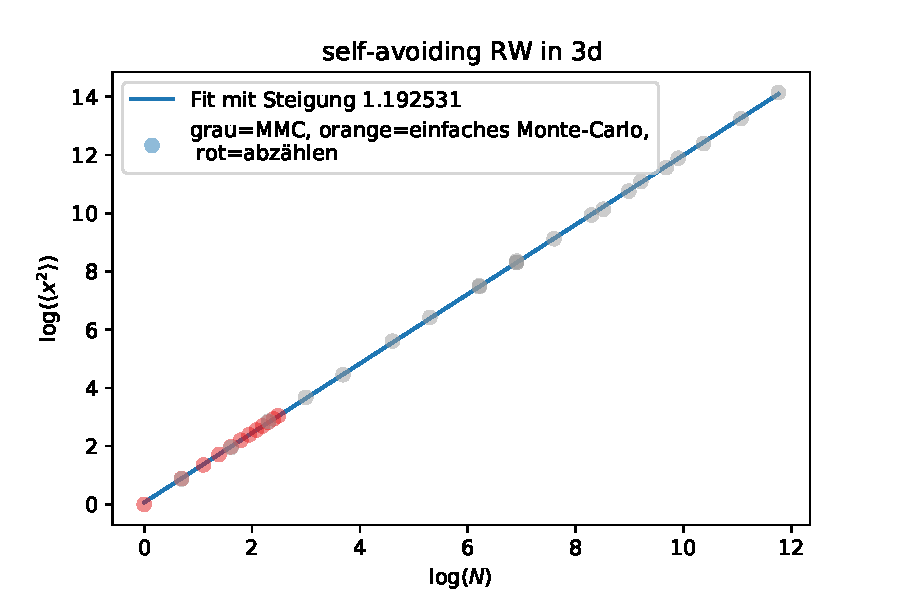
\includegraphics[width=1.2\textwidth]{saw/saw3d.pdf}
				\caption{loglog-Plot der mittleren quadratischen Abweichung als Funktion der Länge $N$ (eigene Berechnung)}
			\end{figure}
		\end{column}
		\begin{column}[]{.5\textwidth}
			\tiny
			\begin{table}
				\begin{tabular}{|l|l|l|}
					\hline
					$N$&$\left<R^2\right>$ (95\%) MC& $\left<R^2\right>$ Abzählen\\ \hline
					2&2.40035 (0.00201479)& 2.4\\ \hline
					3&3.87449 (0.0063882)& 3.88\\ \hline
					4&5.54665 (0.0118491)& 5.55372\\ \hline
					5&7.23051 (0.0179694)& 7.2343\\ \hline
					6&9.05697 (0.0242037)& 9.07054\\ \hline
					7&10.8752 (0.0306989)& 10.8972\\ \hline
					8&12.8691 (0.0419492)& 12.8451\\ \hline
					9&14.7818 (0.0493571)& 14.7806\\ \hline
					10&16.8283 (0.0578437)& 16.8172\\ \hline
					11&18.8972 (0.0693893)& 18.8414\\ \hline
					12&20.9687 (0.0797028)& 20.9528\\ \hline
					50&115.886 (0.610594)&\\ \hline
					100&264.892 (1.51423)&\\ \hline
					200&605.564 (3.67205)&\\ \hline
					500&1780.78 (12.4021)&\\ \hline
					1000&4040.07 (30.7672)&\\ \hline
					2000&9189.7 (77.258)&\\ \hline
					4000&20798 (188.555)&\\ \hline
					8000&46932.3 (405.325)&\\ \hline
					16000&106369 (963.302)&\\ \hline
					32000&241757 (2348.76)&\\ \hline
					64000&560815 (5617.45)&\\ \hline
					128000&1.39791e+06 (16746.3)&\\ \hline
				\end{tabular}
			\end{table}
		\end{column}
	\end{columns}
\end{frame}
\begin{frame}
	\frametitle{Quellen}
	\begin{enumerate}[ {[}1{]} ]
		\tiny
		\item Gardiner, C. W. (1985). Handbook of stochastic methods (Vol. 3, pp. 2-20). Berlin: springer.
		\item Demtröder, W., Experimentalphysik, I. (2006). Mechanik und Wärme. Springer.
		\item Klafter, J., \& Sokolov, I. M. (2005). Anomalous diffusion spreads its wings. Physics world, 18(8), 29.
		\item Ritchie, K., Shan, X. Y., Kondo, J., Iwasawa, K., Fujiwara, T., \& Kusumi, A. (2005). Detection of non-Brownian diffusion in the cell membrane in single molecule tracking. Biophysical journal, 88(3), 2266-2277.
		\item Kusumi, A., \& Sako, Y. (1996). Cell surface organization by the membrane skeleton. Current opinion in cell biology, 8(4), 566-574.
		\item Ramos-Fernández, G., Mateos, J. L., Miramontes, O., Cocho, G., Larralde, H., \& Ayala-Orozco, B. (2004). Lévy walk patterns in the foraging movements of spider monkeys (Ateles geoffroyi). Behavioral ecology and Sociobiology, 55(3), 223-230.
		\item Spiegel O, Getz WM, Nathan R (2013) Factors influencing foraging search efficiency: Why do scarce lappet-faced vultures outperform ubiquitous white-backed vultures? The American Naturalist 181(5), E102-115
		\item Spiegel, O., Harel, R., Centeno-Cuadros, A., Hatzofe, O., Getz, W. M., \& Nathan, R. (2015). Moving beyond curve fitting: using complementary data to assess alternative explanations for long movements of three vulture species. The American Naturalist, 185(2), E44-E54.
		\item Schütz, G. M., \& Trimper, S. (2004). Elephants can always remember: Exact long-range memory effects in a non-Markovian random walk. Physical Review E, 70(4), 045101.
		\item Madras, N., \& Slade, G. (2013). The self-avoiding walk. Springer Science \& Business Media.
		\item Madras, N., \& Sokal, A. D. (1988). The pivot algorithm: a highly efficient Monte Carlo method for the self-avoiding walk. Journal of Statistical Physics, 50(1-2), 109-186.
		\item Lal, M. (1969). ‘Monte Carlo’computer simulation of chain molecules. I. Molecular physics, 17(1), 57-64.
	\end{enumerate}
\end{frame}

\end{document}